\section{Why It Works: A White-Box Analysis}
\label{sec:analysis}
Because \method changes only the mask, the source of its advantage is observable off the selection. Refreshing perturbations at each operating point limits the extrapolation each step performs (Sec.~\ref{sec:continuation}), and the resulting edge traces to a concrete choice of what to remove (Sec.~\ref{sec:whitebox}).

\subsection{The Role of $K$}
\label{sec:continuation}
Splitting the budget into $K$ re-estimated steps directly attacks the trust-region violation.
Perplexity is \emph{monotone} in $K$ ($1497\!\to\!1205\!\to\!823\!\to\!389$ across $K{=}1,2,4,8$ at $\rho{=}0.5$, a $3.9\times$ reduction), the diminishing-returns signature the $1/K^2$ bound predicts (Prop.~\ref{prop:k2}); we fix $K{=}8$ and treat step placement as a secondary knob that helps the sharpest-collapsing models.
The mechanism is directly logged: the revived first-order drift mass $\sum_u|g^{(k)}_u|$ is \emph{zero} at the dense step and grows along the path, faster at higher sparsity, exactly the signal one-shot structurally cannot see and precisely where it fails.

\subsection{What Is Pruned}
\label{sec:whitebox}
Two findings read directly off the mask (Fig.~\ref{fig:whitebox}). \textbf{(i)
\method prunes attention heads that one-shot leaves intact.} One-shot's dense-point quadratic rates every
attention head as critical and removes essentially \emph{zero} ($\le1$ head at every ratio), cutting almost
exclusively FFN groups; re-estimating along the path reveals heads that \emph{become} cheap to remove, and \method
prunes $47/71/156$ heads at $\rho{=}0.2/0.3/0.5$. This freed budget is the source of its perplexity edge,
and the selected masks are substantially different from one-shot (Jaccard $.24$--$.55$), a genuine reorganization rather than a refinement. \textbf{(ii) The
\emph{schedule} resolves the attention trade-off.} Pruning heads aids language modeling but, done too aggressively against a stale early linearization, can cost BoolQ at one moderate-sparsity cell ($\rho{=}0.3$); the \textbf{optional schedule refinement} re-evaluates each head against a freshly perturbed operating point near the target and lifts BoolQ to $\mathbf{.676}$ (\emph{above} one-shot's $.629$) while \emph{also} improving perplexity ($14.1$ vs.\ $19.9$), reaching the favorable corner of the perplexity$\leftrightarrow$BoolQ front (Fig.~\ref{fig:whitebox}b) on which one-shot is dominated.

\begin{figure}[t]
\centering
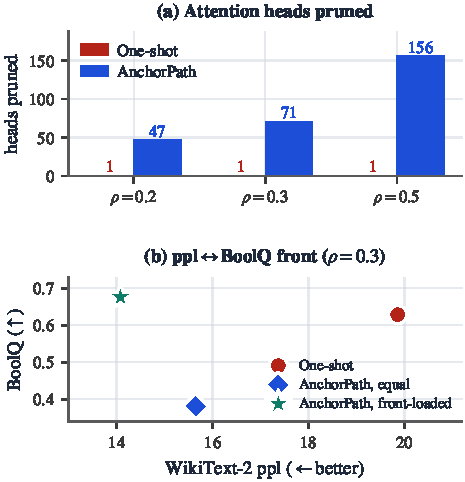
\includegraphics[width=0.7\columnwidth]{figs/fig_whitebox.pdf}
\caption{\textbf{A white-box account of the edge} (LLaMA-2-7B). (a) \method prunes many attention heads where one-shot prunes essentially none. (b) On the perplexity$\leftrightarrow$BoolQ plane the front-loaded schedule reaches the favorable corner, on which one-shot is dominated.}
\label{fig:whitebox}
\end{figure}